\documentclass[dvipdfmx,uplatex]{jsarticle}

%% Packages
\usepackage{graphicx,color,hyperref}
\usepackage{algorithm}
\usepackage{algorithmic}
\usepackage{url}
\usepackage{lscape}
\usepackage{mathtools}
\usepackage{here}
\usepackage{amsmath,amssymb,amsfonts}
\usepackage{amsthm}
\usepackage{tikz}
\usepackage{tcolorbox}
\usepackage{pxjahyper}

%% Theorem Styles
\newtheorem{theorem}{定理}
\newtheorem{proposition}{命題}
\newtheorem{cor}{系}
\newtheorem{definition}{定義}
\newtheorem{problem}{問題}
\theoremstyle{remark}
\newtheorem{remark}{注意}
\newtheorem{requirement}{条件}

%% Environment (Colorful Box)
\newenvironment{simplebox}{
    \begin{tcolorbox}[
        fonttitle=\bfseries,
    ]
}{
    \end{tcolorbox}
}

\newenvironment{method}[1]{
    \begin{tcolorbox}[
        colframe=green!50!black,
        colback=green!50!black!10!white,
        colbacktitle=green!50!black!40!white,
        coltitle=black,
        fonttitle=\bfseries,
        title={#1}
    ]
}{
    \end{tcolorbox}
}

\newenvironment{experiment}[1]{
    \begin{tcolorbox}[
        colframe=violet,
        colback=violet!10!white,
        colbacktitle=violet!40!white,
        coltitle=black,
        fonttitle=\bfseries,
        title={#1}
    ]
}{
    \end{tcolorbox}
}

\newenvironment{kansou}{
    \begin{tcolorbox}[
        colframe=brown,
        colback=brown!10!white,
        colbacktitle=brown!40!white,
        coltitle=black,fonttitle=\bfseries
    ]
}{
    \end{tcolorbox}
}

%% Title
\title{Is Long Context All You Need? Leveraging LLM’s Extended
Context for NL2SQL}
\author{\empty}
\date{\empty}

%% Document body
\begin{document}
\maketitle

\begin{itemize}
    \item Link: \url{https://www.vldb.org/pvldb/vol18/p2735-ozcan.pdf}
    \item Conference: VLDB2025
    \item Arxiv: \url{https://arxiv.org/pdf/2501.12372}
\end{itemize}

\section{概要}
\begin{simplebox}
\begin{itemize}
    \item NL2SQLにおけて、LLMが長いコンテキストウィンドウを持つことの効果を調査した。仮説はコンテキストウィンドウが長いほどスキーマ情報や、列の値などの値を多く含めることができ、性能が向上するというものである。
    \item 実験により以下のような知見を得た。
    \begin{itemize}
        \item 正しいテーブル、カラムをコンテキストに含める必要があり、多くの無関係なテーブル情報が入っていても問題はない。
        \item 多くの質問の類似度によって選択された例を追加しても、NL2SQL精度が大幅に向上されるわけではなく、同じターゲットテーブルからの例を追加する方が効果的である。
        \item レイテンシはコンテキストサイズに線形に比例してぞうかするため、レイテンシと精度向上の間には明確なトレードオフが存在する。
    \end{itemize}
\end{itemize}
\end{simplebox}

\section{手法}
\begin{method}{Long Context Prompting}
\begin{itemize}
    \item 長いコンテキストの活用法を提案する、本研究では「SQL生成、修正、検証」の3つのステップを通じて長いコンテキストの効果を検証する。
    \item Generate
    \begin{itemize}
        \item すべてのデータベーステーブルを用いたスキーマリンキング: RAGなどで関連するテーブルを選択するのではなく、すべてのテーブルをコンテキストに含める。
        \item  カラム記述とサンプル値を含める: 各カラムの説明と、サンプル値を含めることで、LLMがカラムの意味を理解しやすくする。
        \item ユーザからの追加の指示やヒント: ユーザとの複数ターンの対話を通じて得られたヒントなどを含める。
        \item 合成SQLクエリの例を含める: 生成したSQLサンプルの例を数十から数百個含める。
        \item 関連するSQLiteドキュメントのセクション
    \end{itemize}
    \item Fix and Rewrite: モデルがSQLの実行結果に基づいてSQLを修正することを許すようにする
    \item Verify: SQLの実行結果が期待通りであることを確認する   
\end{itemize}
\end{method}

\section{LongContextLLMの評価}
\begin{experiment}{評価設定}
\begin{itemize}
    \item モデル: GCP gemini APIを利用し、gemini-1.5-pro-002, gemini-1.5-flash-002 を利用する.
    \item ベンチマークデータセット: Bird, Spider, KaggleDBQA, Beaver
    \item 性能、コスト指標: 実行精度、リクエストあたりのトークン数、レイテンシ
\end{itemize}
\end{experiment}

\begin{figure}
    \centering
    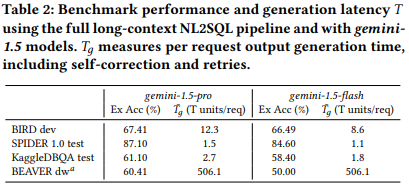
\includegraphics[width=0.7\textwidth]{img/long-context-nl2sql/result.png}
    \caption{Long Context LLMの評価結果}
    \label{fig:full-result}
\end{figure}

\begin{figure}
    \centering
    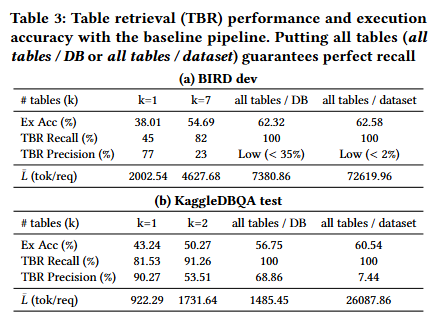
\includegraphics[width=0.7\textwidth]{img/long-context-nl2sql/all-table.png}
    \caption{全テーブルを用いたスキーマリンキングの効果}
    \label{fig:all-table}
\end{figure}

\begin{experiment}{実験結果}
\begin{itemize}
    \item ベンチマーク評価
    \begin{itemize}
        \item 各データセットにおける評価結果を図\ref{fig:full-result}に示す。この結果は前節のすべてのコンテキスト情報を入れた場合のものである。
        \item BeaverベンチマークはDWHのようなユースケースを想定されており、他のベンチマークよりもJOINが必要なクエリがおおく、テーブルの数も多いため、他のベンチマークよりも精度が低い。
    \end{itemize}
    \item 全テーブルを用いたスキーマリンキングの効果
    \begin{itemize}
        \item 図\ref{fig:all-table}に示すように、全テーブルを用いたスキーマリンキングは効果的である。この結果は大量の情報を入れても、LLMが必要な情報をうまく抽出できることを示している。
    \end{itemize}
    \item 合成SQLクエリの例の効果
    \begin{itemize}
        \item 無関係な例を含めすぎると精度が下がる場合もある。
        \item 合成SQLクエリをたくさんいれると精度向上に寄与する、とくに同じテーブルからのトレーニングサンプルがない場合は効果的である。
    \end{itemize}
    \item 自己修正の効果
    \begin{itemize}
        \item 正しいSQLが生成されたが、結果が空であったときに列値のサンプルリストを提示することで自己修正させる。自己修正によって修正が行われるが精度は数\%程度しか増加せず、その割には必要な入力トークンが多い。
        \item ユーザへの追加質問を行いスキーマ情報をフィルタリングする、この場合は数\%程度精度が向上し、必要な入力トークン数もそれほど多くない。
    \end{itemize}
    \item SQLiteのドキュメントの効果
    \begin{itemize}
        \item ほとんど効果ない、それはおそらくすでにモデルが知識としてもっているため。
    \end{itemize}
    \item コンテキストとレイテンシの関係
    \begin{itemize}
        \item コンテキストサイズが大きくなると、レイテンシもほぼ線形に増加する。
        \item また興味深い現象としてコンテキストサイズが32kを超えるとレイテンシが大きく増加する、それはLLMの推論が複数のホストに分散されてキューイングが生じるためと考えられる。
    \end{itemize}
\end{itemize}
\end{experiment}

\begin{experiment}{Ablation Study}
コンテキスト情報を一つずつ追加する追加実験を行った。
異なる種類のコンテキスト情報が異なる質問タイプに有効であることが示された。
\begin{itemize}
    \item 追加のサンプル値は複雑な質問やあいまいな質問に有効。
    \item SQLの合成例は簡単な質問に有効だが、難しい質問では性能低下の場合もある。
    \item ユーザへの追加質問によるヒントは特に重要で正確なSQL生成に大きく寄与する。
\end{itemize}
\end{experiment}

\section{感想}
\begin{kansou}
\begin{itemize}
  \item Gemini1.5proは古くないか?とは思った。
  \item テーブルスキーマをすべてプロンプトにいれてもそこそこ機能するという点は面白いと思った。コンテキスト長が長くなりすぎてコスト的な問題が発生するため、実際のアプリケーションで使うには工夫が必要そう。
  \item 入力トークン長がある閾値より大きくなるとレイテンシが大きく増加するというのはおもしろい、入力トークンがある程度長くなるとAPIの裏側でキューイングなど発生してレイテンシとその分散が大きくなるというのは納得感がある。
\end{itemize}
\end{kansou}

% self-consistency, self-correction, schema-linkingは重要な技術かも

\end{document}